\section{Applications utilisées par SPIE Sud-Est}

\begin{figure}[H]
    \label{fig-applis-spie}
    \noindent\makebox[\textwidth]{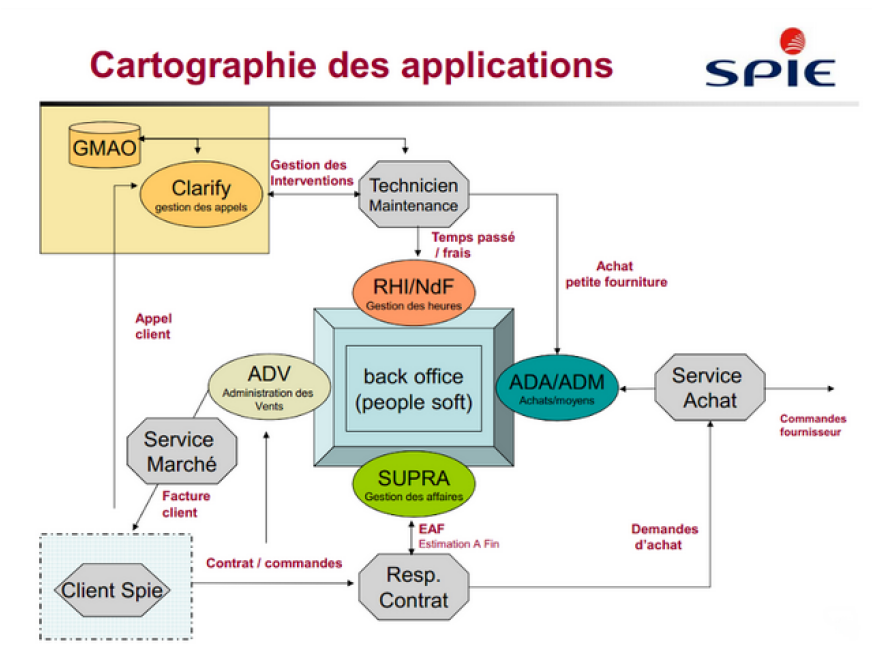
\includegraphics[width=10cm]{figures/applications_spie.png}}
    \caption{Cartographie applicative de SPIE Sud-Est}
\end{figure}

\subsection{People Soft}
Dévéloppé par Oracle et configuré pour répondre à certains des besoins métiers de SPIE.
\begin{description}
    \item \bf{Finalité :} Gestion centralisé de certains processus métiers. \\
    \item \bf{Fonctions :}
    \begin{itemize}
        \item Système de gestion de resources humaines
        \item Financial Mangagement Solution
        \item Customer Relationship Management
        \item Entreprise Performance Management \\
    \end{itemize}
    \item \bf{Utilisateurs :} Tous les utilisateurs des fonctions ci-dessus. \\
    \item \bf{Contraintes :} Ne couvre pas tous les besoins métiers de SPIE et oblige SPIE à avoir d’autres applications spécifique.
\end{description}

\subsection{ADV}
Développement spécifique pour les besoins de SPIE.
\begin{description}
    \item \bf{Finalité :} Administration des ventes. \\
    \item \bf{Fonctions :}
    \begin{itemize}
        \item Enregistrement des commandes de vente
        \item Gestion de la facturation
    \end{itemize}
\end{description}

\subsection{ADA-ADM}
Développement spécifique pour les besoins de SPIE.
\begin{description}
    \item \bf{Finalité :} Administration des achats / Administration des moyens. \\
    \item \bf{Fonctions :}
    \begin{itemize}
        \item Gestion des achats
        \item Gestion des moyens (véhicules / outillages) \\
    \end{itemize}
    \item \bf{Utilisateurs :} Employés du service achat et du service moyens
\end{description}

\subsection{RHI - NDF}
Développement Spécifique pour les besoins de SPIE.
\begin{description}
    \item \bf{Finalité :} Gestion des heures de paies des employés de SPIE. \\
    \item \bf{Fonctions :}
    \begin{itemize}
        \item Sui du pointage des emplyés
        \item Suivi de l’activité hebdomadaires des techniciens de maintenances (tâches effectées, délai et temps d’intervention)
        \item Gestion des notes de frais (saisis des frais liés aux intervention de maintenance, c’est à dire les déplacements ou bien les déjeuners) \\
    \end{itemize}
    \item \bf{Utilisateurs :} Techniciens de maintenance et service comptable. \\
    \item \bf{Inconvénients :} Le but de ce logiciel est de gérer les heures des techniciens chaque semaine. Cependant, il n’est pas très souple et est utilisé en parallèle de macros excel. \\
\end{description}

\bf{Observations :} Il faudra fournir un logiciel de meilleur qualité permettant de s’affranchir de Excel.


\subsection{SUPRA}
Développement spécifique pour les besoins de SPIE.
\begin{description}
    \item \bf{Finalité :} Suivi et Gestion pour le responsable d’affaires. \\
    \item \bf{Fonctions :}
    \begin{itemize}
        \item Accès à l’ensemble des informations relatives aux projets du Restponsable d’affaires
        \item Commandes
        \item Dépenses engagées
        \item Factures de fournisseurs
        \item Données internes à l’équipe (heures dépensées par les équipes et coûts associés) \\
    \end{itemize}
    \item \bf{Utilisateurs :} Responsable d’affaires. \\
    \item \bf{Inconvénients :} SUPRA est un application très ancienne héritant de l’ancien ERP de SPIE. Elle a donc subie de nombreuses modifications et présente des dysfonctionnements liées à ces évolutions. \\ répétées. 
\end{description}

\bf{Observations :} Certaines fonctions sont aussi présentes dans d’autres outils, il faudrait essayer de faire un peu de “ménage” pour garder que ce qui n’est pas répliqué ailleurs.


\subsection{Clarify}
Développement spécifique pour les besoins de SPIE.
\begin{description}
    \item \bf{Finalité :} Gestion des appels et des demandes d’interventions. \\
    \item \bf{Fonctions :} 
    \begin{itemize}
        \item Gestion (classifications/commentaires) et enregistrement des appels
        \item Traitement des demandes d’intervention et envoi éventuel d’une équipe de maintenance \\
    \end{itemize}
    \item \bf{Utilisateurs :} Agent centre d’appels, responsale de maintenance, techniciens de maintenance
\end{description}

\subsection{Conclusion}

Globalement, l’architecture applicative de la gestion de la maintenance souffre d’une segmentation importance ainsi que de trop nombreux flux. Il peut être nécessaire d’essayer de diminuer la taille de l’architecture applicative en essayant des alternatives qui pourraient couvrir l’ensemble des besoins de SPIE.

\section{Architecture technique de SPIE Sud-Est}

SPIE Sud-Est n'a pas accepté de diffuser les informations concernant les architectures techniques existantes. Nous sommes donc dans l'impossibilité de détailler cette dimension de l'étude de l'existant.